\chapter{Security}
\url{https://docs.microsoft.com/en-us/previous-versions/windows/it-pro/windows-server-2008-r2-and-2008/cc772066(v=ws.10)}

\section{User Account Control (UAC)}


\label{windows_knowledge:fundamentals:security:uac}

\href{https://docs.microsoft.com/en-us/windows/security/identity-protection/user-account-control/how-user-account-control-works}{User
Account Control (UAC)}~\ref{windows_knowledge:ad:rights_privileges:uac}
 is a Windows security feature that forces any new process to run in the
 security context of a non-privileged account by default. This policy applies
 to processes started by any user, including administrators themselves. The
 idea is that we can't solely rely on the user's identity to determine if some
 actions should be authorized.

 \subsection{UAC elevation}
Each app that requires the administrator access token must prompt for consent.
The one exception is the relationship that exists between parent and child
processes. Child processes inherit the user's access token from the parent
process. Both the parent and child processes, however, must have the same
integrity level.

When a standard user attempts to run an app that requires an administrator
access token, UAC requires that the user provide valid administrator
credentials.

 \subsection{Mandatory Integrity Controls and Integrity level}
\href{https://docs.microsoft.com/en-us/windows/win32/secauthz/mandatory-integrity-control}{Mandatory
Integrity Control (MIC)} provides a mechanism for controlling access to
securable objects. This mechanism is in addition to discretionary access
control and evaluates access before access checks against an object's
discretionary access control list (DACL) are evaluated. 

MIC uses \emph{integrity levels} and mandatory policy to evaluate access. Security
principals and securable objects are assigned integrity levels that determine
their levels of protection or access. In general terms, users or processes with
a higher IL access token will be able to access resources with lower or equal
ILs.

The following 4 ILs are used by Windows, ordered from lowest to highest:
\begin{tabularx}{\linewidth}{|l|X|}
    \hline
Integrity Level	& Use \\
    \hline
Low	& Generally used for interaction with the Internet (i.e. Internet
Explorer). Has very limited permissions. \\
    \hline
Medium &	Assigned to standard users and Administrators' filtered tokens.\\
    \hline
High&	Used by Administrators' elevated tokens if UAC is enabled. If UAC is
disabled, all administrators will always use a high IL token. \\
    \hline
System &	Reserved for system use.\\
    \hline
\end{tabularx}

When a process requires to access a resource, it will inherit the calling user's access token and its associated IL. The same occurs if a process forks a child.

Regarding tokens:
\begin{itemize}
    \item token of a non-administrator has a medium IL
    \item Filtered token~\ref{win:filtered-token} of an Administrator has a
        medium IL
    \item Elevated token of an Administrator has a high IL
\end{itemize}

\subsection{UAC settings}
UAC can be configured to run at four different notification levels:
\begin{itemize}
    \item {\bf Always notify}: Notify and prompt the user for authorization
        when making changes to Windows settings or when a program tries to
        install applications or make changes to the computer.
    \item {\bf Notify me only when programs try to make changes to my
            computer}: Notify and prompt the user for authorization when a
            program tries to install applications or make changes to the
            computer. Administrators won't be prompted when changing Windows
            settings.
    \item {\bf Notify me only when programs try to make changes to my computer
        (do not dim my desktop)}: Same as above, but won't run the UAC prompt
        on a secure desktop.
    \item {\bf Never notify}: Disable UAC prompt. Administrators will run everything using a high privilege token.
\end{itemize}

By default, UAC is configured on the Notify me only when programs try to make
changes to my computer level.

From an attacker's perspective, the three lower security levels are equivalent,
and only the Always notify setting presents a difference.
\subsubsection{Security policy settings}
See
\href{https://docs.microsoft.com/en-us/windows/security/identity-protection/user-account-control/user-account-control-security-policy-settings}{Microsoft
 documentation} for more information.

\subsubsection{Group Policy settings}
See \href{https://docs.microsoft.com/en-us/windows/security/identity-protection/user-account-control/user-account-control-group-policy-and-registry-key-settings#group-policy-settings}{Microsoft
 documentation} for more information.

\subsubsection{Registry key settings}

 The parameters responsible for the behavior of User Account Control are
 located under the registry key 
 \begin{verbatim}
 HKLM\SOFTWARE\Microsoft\Windows\CurrentVersion\Policies\System
 \end{verbatim}

 See
 \href{https://docs.microsoft.com/en-us/windows/security/identity-protection/user-account-control/user-account-control-group-policy-and-registry-key-settings#registry-key-settings}{Microsoft
 documentation} for more information.

\subsection{Application Information Service}
At the heart of UAC, there is the Application Information Service or Appinfo. Whenever a user requires elevation, the following occurs:
\begin{enumerate}
        \item The user requests to run an application as administrator.
        \item A ShellExecute API call is made using the runas verb.
        \item The request gets forwarded to Appinfo to handle elevation.
        \item The application manifest is checked to see if AutoElevation is allowed (more on this later).
        \item Appinfo executes consent.exe, which shows the UAC prompt on a secure desktop. A secure desktop is simply a separate desktop that isolates processes from whatever is running in the actual user's desktop to avoid other processes from tampering with the UAC prompt in any way.
        \item If the user gives consent to run the application as administrator, the Appinfo service will execute the request using a user's Elevated Token. Appinfo will then set the parent process ID of the new process to point to the shell from which elevation was requested.
\end{enumerate}

    The following diagram, adapted from the source here, illustrates how UAC works.

\begin{figure}
  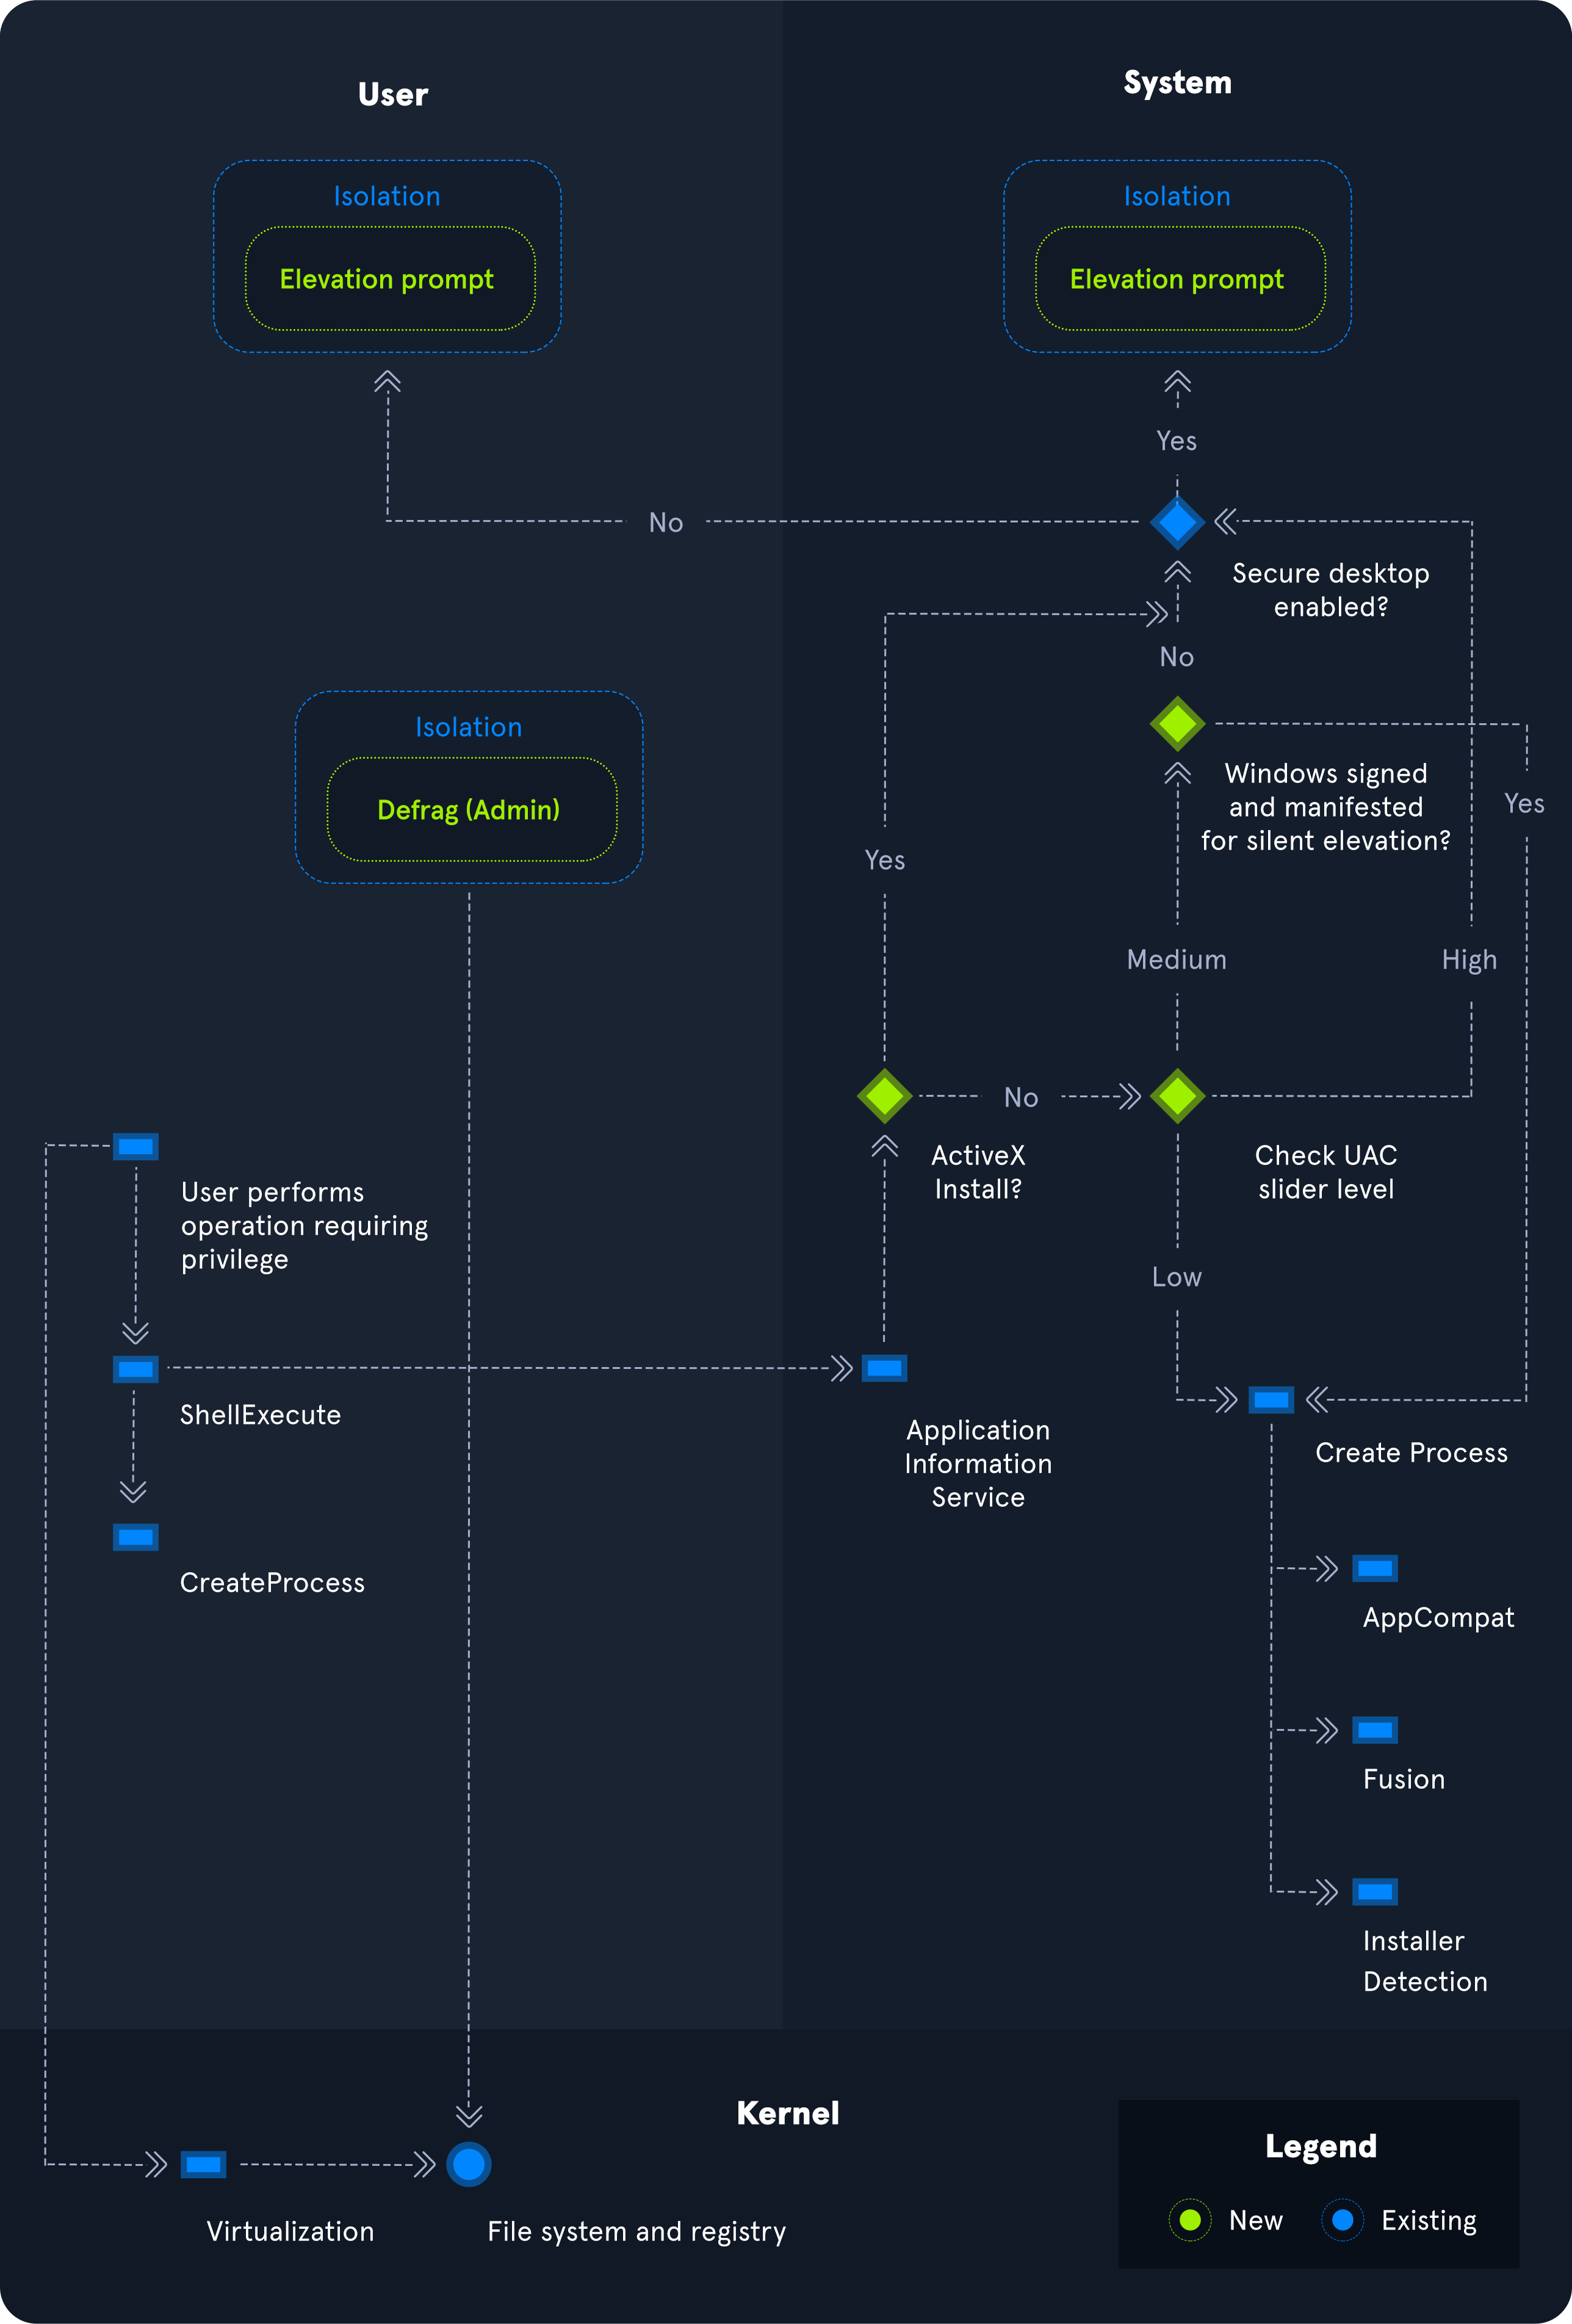
\includegraphics[width=\linewidth]{windows_knowledge/security/images/uac_architecture.png}
  \caption{UAC architecture}
  \label{fig:uac-architecture}
\end{figure}


\subsection{Auto-elevating processes}

Some programs are autoelevated automatically if the user belongs to the
administrator group. 

To bypass the UAC (elevate from medium integrity level to high) some
attackers use this kind of binaries to execute arbitrary code because it will
be executed from a High level integrity process.


For an application, some requirements need to be met to
auto-elevate:
\begin{itemize}
    \item The binary has to be signed by Microsoft Publisher 
    \item the binary must be contained in a trusted directory (like \verb+%SystemRoot%/System32/+ or
    \verb+%ProgramFiles%/+)
\end{itemize}

Depending on the type of application, additional requirements may apply:

\begin{itemize}
    \item Executable files (.exe) must declare the autoElevate element inside
        their manifests.  \verb+sigcheck.exey+ from Sysinternals allow to check
        the Manifest of a binary.

    \item mmc.exe will auto elevate depending on the .msc snap-in that the user requests. Most of the .msc files included with Windows will auto elevate.
    \item Windows keeps an additional list of executables that auto elevate even when not requested in the manifest. This list includes pkgmgr.exe and spinstall.exe, for example.
    \item COM objects can also request auto-elevation by configuring some
        registry keys (See
        \href{https://docs.microsoft.com/en-us/windows/win32/com/the-com-elevation-moniker}{Windows
    documentation}).
\end{itemize}


\section{Registry}
\index{Windows!registry}
\label{win:registry}

The \href{https://en.wikipedia.org/wiki/Windows_Registry}{Registry} is a
hierarchical database in Windows critical for the operating system. It stores
low-level settings for the Windows operating system and applications that
choose to use it. It is divided into computer-specific and user-specific data.


The \verb+regedit+ command allow to view/edit it.

The tree-structure consists of main folders (root keys) in which subfolders
(subkeys) with their entries/files (values) are located. There are 11 different
types of values that can be entered in a subkey.

Each folder under i\verb+Computer+ is a key. The root keys all start with
\verb+HKEY+. A key such as \verb+HKEY-LOCAL-MACHINE+ is abbreviated to
i\verb+HKLM+. 

\verb+HKLM+ contains all settings that are relevant to the local system. This
root key contains six subkeys like \verb+SAM+, \verb+SECURITY+, \verb+SYSTEM+,
\verb+SOFTWARE+, \verb+HARDWARE+, and \verb+BCD+, loaded into memory at boot
time (except HARDWARE which is dynamically loaded).

The entire system registry is stored in several files on the operating system.
You can find these under \verb+C:\Windows\System32\Config\+.

The user-specific registry hive (\verb+HKCU+) is stored in the user folder
(i.e., \verb+C:\Windows\Users\<USERNAME>\Ntuser.dat+).

\section{Run and RunOnce Registry Keys}

There are also so-called \gls{win:registry-hive}, which contain a logical group
of keys, subkeys, and values to support software and files loaded into memory
when the operating system is started or a user logs in. These hives are useful
for maintaining access to the system. These are called
\href{https://docs.microsoft.com/en-us/windows/win32/setupapi/run-and-runonce-registry-keys}{Run
and RunOnce registry keys}.

\section{AppLocker (Application Whitelisting)}
\label{windowd_knowledge:fundamentals:security:applocker}
An application whitelist is a list of approved software applications or executables allowed to be present and run on a system. The goal is to protect the environment from harmful malware and unapproved software that does not align with the specific business needs of an organization. Implementing an enforced whitelist can be a challenge, especially in a large network. An organization should implement a whitelist in audit mode initially to make sure that all necessary applications are whitelisted and not blocked by an error of omission, which can cause more problems than it fixes.

Blacklisting, in contrast, specifies a list of harmful or disallowed software/applications to block, and all others are allowed to run/be installed. Whitelisting is based on a "zero trust" principle in which all software/applications are deemed "bad" except for those specifically allowed. Maintaining a whitelist generally has less overheard as a system administrator will only need to specify what is allowed and not constantly update a "blacklist" with new malicious applications.

Whitelisting is recommended by organizations such as NIST, especially in high-security environments.

\href{https://docs.microsoft.com/en-us/windows/security/threat-protection/windows-defender-application-control/applocker/applocker-overview}{AppLocker} is Microsoft's application whitelisting solution and was first introduced in Windows 7. AppLocker gives system administrators control over which applications and files users can run. It gives granular control over executables, scripts, Windows installer files, DLLs, packaged apps, and packed app installers.

It allows for creating rules based on file attributes such as the publisher's name (which can be derived from the digital signature), product name, file name, and version. Rules can also be set up based on file paths and hashes. Rules can be applied to either security groups or individual users, based on the business need. AppLocker can be deployed in audit mode first to test the impact before enforcing all of the rules.


\section{Local Group Policy}
Group Policy allows administrators to set, configure, and adjust a variety of settings. In a domain environment, group policies are pushed down from a Domain Controller onto all domain-joined machines that Group Policy objects (GPOs) are linked to. These settings can also be defined on individual machines using Local Group Policy.

Group Policy can be configured locally, in both domain environments and non-domain environments. Local Group Policy can be used to tweak certain graphical and network settings that are otherwise not accessible via the Control Panel. It can also be used to lock down an individual computer policy with stringent security settings, such as only allowing certain programs to be installed/run or enforcing strict user account password requirements.

We can open the Local Group Policy Editor by opening the Start menu and typing
\verb+gpedit.msc+. The editor is split into two categories under Local Computer
Policy - \emph{Computer Configuration} and \emph{User Configuration}.

 
Local Group Policy Editor enables fine-tuned account auditing and configure
AppLocker.

\section{Microsoft Defender}
\label{windowd_knowledge:fundamentals:security:defender}
\href{https://en.wikipedia.org/wiki/Microsoft_Defender}{Microsoft Defender}, formerly known as Windows Defender, is built-in antivirus that ships for free with Windows operating systems. It was first released as a downloadable anti-spyware tool for Windows XP and Server 2003. Defender started coming prepackaged as part of the operating system with Windows Vista/Server 2008. The program was renamed to Windows Defender Antivirus with the Windows 10 Creators Update.

Defender comes with several features such as real-time protection, which protects the device from known threats in real-time and cloud-delivered protection, which works in conjunction with automatic sample submission to upload suspicious files for analysis. When files are submitted to the cloud protection service, they are "locked" to prevent any potentially malicious behavior until the analysis is complete. Another feature is Tamper Protection, which prevents security settings from being changed through the Registry, PowerShell cmdlets, or group policy.

Windows Defender is managed from the Security Center, from which a variety of additional security features and settings can be enabled and managed.

Real-time protection settings can be tweaked to add files, folders, and memory areas to controlled folder access to prevent unauthorized changes. We can also add files or folders to an exclusion list, so they are not scanned. An example would be excluding a folder of tools used for penetration testing from scanning as they will be flagged malicious and quarantined or removed from the system. Controlled folder access is Defender's built-in Ransomware protection.

We can use the PowerShell cmdlet \verb+Get-MpComputerStatus+ to check which protection settings are enabled.

Windows Defender is not without its flaws and should be part of a defense-in-depth strategy built around core principles of configuration and patch management, not treated as a silver bullet for protecting our systems. Definitions are updated constantly, and new versions of Windows Defender are built-in to major operating releases such as Windows 10, version 1909, which is the most recent version at the time of writing.

Windows Defender will pick up payloads from common open-source frameworks such as Metasploit or unaltered versions of tools such as Mimikatz.

\section{Windows Credential Manager and Windows Vault}
\label{windowd_knowledge:fundamentals:security:cedential_manager}
\label{windowd_knowledge:fundamentals:security:cedential_vault}

Windows includes a feature called {\bf credential manager}. It stores frequently used
passwords so you can easily access and manage. There is  the ability to back up
or restore this information. The default storage vault for the credential
manager information is the {\bf Windows Vault}. 

the Windows Vault stores user credentials for servers, wesbites and other
programs that Windows can log in the users automatically. which means that any
Windows application that needs credentials to access a resource (server or a
website) can make use of this Credential Manager and Windows Vault and use the
credentials supplied instead of users entering the username and password all
the time.


So, if your application wants to make use of the vault, it should somehow
communicate with the credential manager and request the credentials for that
resource from the default storage vault.

Example of usage: 
\begin{verbatim}
runas /user:WORKGROUP\Administrator /savecred 'cmd.exe...
\end{verbatim}

These information are stored in files have the " System files" attribute,
\begin{verbatim}
%userprofile%\AppData\Local\Microsoft\Vault
%userprofile%\AppData\Local\Microsoft\Credentials
%userprofile%\AppData\Roaming\Microsoft\Vault
%userprofile%\AppData\Roaming\Microsoft\Credentials
\end{verbatim}

\verb+cmdkey.exe+ is a tool used to manage user credential

\section{Data Protection API (DPAIP)}
\href{https://docs.microsoft.com/en-us/previous-versions/ms995355(v=msdn.10)}{Data
ProtectionAPI (DPAPI)} is a simple cryptographic application programming
interface available as a built-in component in Windows 2000 and later versions
of Microsoft Windows operating systems. In theory, the Data Protection API can
enable symmetric encryption of any kind of data; in practice, its primary use
in the Windows operating system is to perform symmetric encryption of
asymmetric private keys, using a user or system secret as a significant
contribution of entropy. A detailed analysis of DPAPI inner-workings was
published in 2011 by
\href{https://learn.microsoft.com/en-us/previous-versions/ms995355(v%3Dmsdn.10)}{Bursztein et al}.

For nearly all cryptosystems, one of the most difficult challenges is "key
management" – in part, how to securely store the decryption key. If the key is
stored in plain text, then any user that can access the key can access the
encrypted data. If the key is to be encrypted, another key is needed, and so
on. DPAPI allows developers to encrypt keys using a symmetric key derived from
the user's logon secrets, or in the case of system encryption, using the
system's domain authentication secrets.

The DPAPI keys used for encrypting the user's RSA keys are stored under 
\verb+%APPDATA%\Microsoft\Protect\{SID}+ directory, where \verb+{SID}+ is the
Security Identifier of that user. The DPAPI key is stored in the same file as
the master key that protects the users private keys. It usually is 64 bytes of
random data. 

These files have the " System files" attribute, and so \verb+DIR /AS+ must be used

\begin{verbatim}
Get-ChildItem  C:\Users\USER\AppData\Roaming\Microsoft\Protect\
Get-ChildItem  C:\Users\USER\AppData\Local\Microsoft\Protect\

dir %appdata%\Microsoft\Protect\ /s 
dir %localappdata%\Microsoft\Protect\ /s 

\end{verbatim}

DPAPI doesn't store any persistent data for itself; instead, it simply receives
plaintext and returns ciphertext (or conversely).

DPAPI security relies upon the Windows operating system's ability to protect
the master key and RSA private keys from compromise, which in most attack
scenarios is most highly reliant on the security of the end user's credentials.
A main encryption/decryption key is derived from user's password by PBKDF2
function. Particular data binary large objects can be encrypted in a way that
salt is added and/or an external user-prompted password (aka "Strong Key
Protection") is required. The use of a salt is a per-implementation option –
i.e. under the control of the application developer – and is not controllable
by the end user or system administrator.

Delegated access can be given to keys through the use of a COM+ object. This
enables IIS web servers to use DPAPI. 


PowerShell credentials are often used for scripting and automation tasks as a
way to store encrypted credentials conveniently. The credentials are protected
using DPAPI, which typically means they can only be decrypted by the same user
on the same computer they were created on.

\section{BitLocker}

